\documentclass[a4paper,10pt]{ctexart}
%引用设置使用Bibtex
\usepackage{gbt7714}
\bibliographystyle{gbt7714-numerical}
%页面设置
\usepackage{geometry}
%字体设置
\usepackage{fontspec}
%\setmainfont{Times New Roman}
%定理环境
\usepackage{amsmath}
\numberwithin{equation}{section}
\usepackage{amsthm}
\newtheorem*{definition}{Definition}
\newtheorem{theorem}{Theorem}
\newtheorem{lemma}{Lemma}
\newtheorem*{corollary}{Corollary}
\newtheorem*{proposition}{Proposition}
\newtheorem*{example}{Example}
%数学环境字体
\usepackage{bm}
\usepackage[all]{xy}
%加载 TikZ 用于绘制交换图
\usepackage{tikz-cd}
\usepackage{tikz}
\usepackage{pgfplots}
\newcommand{\tikzdef}{\pgfmathsetmacro} % 在tikzpicture内的foreach循环中定义实数临时变量
%颜色
\usepackage{color,xcolor}

\definecolor{miku}{RGB}{57,197,187}
\definecolor{sakura}{RGB}{255,192,203}
\definecolor{rose}{RGB}{255,228,225}
\definecolor{brown}{RGB}{210,105,30}
\definecolor{lbrown}{RGB}{239,235,224}
\definecolor{bule}{RGB}{0,47,167}
\definecolor{lyellow}{RGB}{250,250,210}
\definecolor{lpurple}{RGB}{255,240,245}
\definecolor{lbule}{RGB}{135,206,250}
\definecolor{gbule}{RGB}{64,224,208}
\definecolor{green}{RGB}{138,200,207}
\definecolor{lgreen}{RGB}{225,255,255}
\definecolor{lorange}{RGB}{248,172,140}
\definecolor{salmon}{RGB}{250,128,114}
\definecolor{burgundy}{rgb}{0.5, 0.0, 0.13}
%链接设置
\usepackage[colorlinks=true,pdfstartview=FitH,linkcolor=blue,anchorcolor=violet, citecolor=magenta]{hyperref} 
%封面
\usepackage{pdfpages}
\usepackage{mathrsfs}
\usepackage{amssymb}
\usepackage{graphicx}
\usepackage{lipsum}
%彩色框
\usepackage{framed}
\usepackage{tcolorbox}
\tcbuselibrary{breakable}
\tcbuselibrary{theorems}
\tcbuselibrary{skins}
\usepackage{colortbl}
\usepackage{float}
\usepackage[export]{adjustbox}
\newtcolorbox[auto counter,number within=section]{notebox}[2][]{%
colback=miku!2!white,
colframe=miku,
coltitle=white,
fonttitle=\bfseries,
rightrule=2pt,
leftrule=2pt,
bottomrule=2pt,
colbacktitle=miku,
theorem style=standard,
breakable,
arc=2pt,
drop fuzzy shadow=black!20!white,
title=Note~\thetcbcounter: #2,#1}
\newtcolorbox[auto counter,number within=section]{markbox}[2][]{%
colback=miku!2!white,
colframe=miku,
coltitle=white,
fonttitle=\bfseries,
rightrule=0pt,
leftrule=0pt,
bottomrule=2pt,
colbacktitle=miku,
theorem style=standard,
breakable,
arc=0pt,
drop fuzzy shadow=black!20!white,
title=Remark~\thetcbcounter: #2,#1}
\newtcolorbox[no counter]{theorems}[2][]{%
width=12cm,
center,
sidebyside,
sidebyside adapt=left,
sidebyside gap=6mm,
sidebyside align=center seam,
colback=burgundy!2!white,
colframe=burgundy,
coltitle=white,
fonttitle=\bfseries,
rightrule=1pt,
leftrule=1pt,
bottomrule=2pt,
colbacktitle=burgundy,
theorem style=standard,
enhanced,
drop fuzzy shadow southeast=black!30!white,
breakable,
arc=0pt,
title=Theorem. #2,#1}
\newtcolorbox[no counter]{definitions}[2][]{%
width=12cm,
center,
colback=lyellow!2!white,
colframe=yellow!3!lyellow,
coltitle=bule,
fonttitle=\bfseries,
rightrule=0pt,
leftrule=1pt,
bottomrule=2pt,
colbacktitle=lyellow,
theorem style=standard,
breakable,
arc=5pt,
enhanced,
drop fuzzy shadow southeast=black!20!white,
title=Definition. #2,#1}
\newtcolorbox[auto counter,number within=section]{corollarys}[2][]{%
colback=lyellow!2!white,
colframe=lyellow,
coltitle=bule,
fonttitle=\bfseries,
rightrule=0pt,
leftrule=1pt,
bottomrule=2pt,
colbacktitle=lyellow,
theorem style=standard,
breakable,
arc=0pt,
enhanced,
drop fuzzy shadow southeast=black!20!white,
title=Corollary~\thetcbcounter: #2,#1}
\newtcolorbox[auto counter,number within=section]{lemmas}[2][]{%
width=12cm,
center,
colback=lyellow!2!white,
colframe=lorange!30!sakura,
coltitle=bule,
fonttitle=\bfseries,
rightrule=0pt,
leftrule=1pt,
bottomrule=2pt,
colbacktitle=lorange!30!sakura,
theorem style=standard,
breakable,
arc=5pt,
enhanced,
drop fuzzy shadow southeast=black!20!white,
title=Lemma. #2,#1}
\newtcolorbox[auto counter,number within=section]{propositions}[2][]{%
width=12cm,
center,
colback=salmon!5,
colframe=salmon!90!black,
coltitle=white,
fonttitle=\bfseries,
rightrule=1pt,
leftrule=1pt,
bottomrule=2pt,
colbacktitle=salmon!90!black,
theorem style=standard,
breakable,
arc=5pt,
enhanced,
drop fuzzy shadow southeast=black!20!white,
title=Proposition. #2,#1}
\newtcolorbox[no counter]{egbox}[2][]{%
width=12cm,
center,
colback=black!5!white,
colframe=black!20!white,
coltitle=black,
fonttitle=\bfseries,
rightrule=1pt,
leftrule=1pt,
bottomrule=2pt,
colbacktitle=black!20!white,
theorem style=standard,
breakable,
arc=0pt,
enhanced,
drop fuzzy shadow southeast=black!20!white,
title=Example. #2,#1}

%\begin{figure}[H]
%\centering
%\includegraphics[center]{pic.png}
%\end{figure}
\geometry{left=3cm,right=3cm,top=2cm,bottom=2cm}
\tcbuselibrary{most}

\usepackage[linesnumbered,ruled,vlined]{algorithm2e}
\usepackage{algorithmic}

\SetKwProg{Fn}{function}{\string:}{}
\newcommand{\forcond}{$i=0$ \KwTo $n$}
\SetKwFunction{FRecurs}{FnRecursive}
\SetKwInput{KwCost}{Cost}

\usepackage{holtpolt}

%自定义设置
\renewcommand{\proofname}{Proof.}
\renewcommand{\contentsname}{ Content }
\newcommand{\image}[2]{
    \centering
    \includegraphics[width={#1}\textwidth]{#2}
}



\newcommand\keywords[1]{\vskip2ex\par\noindent\normalfont{\textbf{关键词}: #1}}
\newcommand{\ekeywords}[1]{\vskip2ex\par\noindent\normalfont{\bfseries Key Words: }#1}
\newcommand{\miku}{\textcolor{miku}}
\newcommand{\sakura}{\textcolor{sakura}}
\newcommand{\brown}{\textcolor{brow}}
\newcommand{\red}{\textcolor{red}}
\newcommand{\blue}{\textcolor{blue}}
\newcommand{\A}{\mathcal{A}}
\newcommand{\C}{\mathbb{C}}
\newcommand{\al}{\alpha}
\newcommand{\sa}{$\sigma$-algebra}
\newcommand{\Bsa}{Borel $\sigma$-algebra}
\newcommand{\F}{\mathcal{F}}
\newcommand{\N}{\mathcal{N}}
\newcommand{\M}{\mathcal{M}}
\newcommand{\m}{ $\mathcal{M}$ }
\newcommand{\B}{\mathcal{B}}
\newcommand{\myP}{\mathcal{P}}
\renewcommand{\bf}[1]{\textbf{#1}}

\newcommand{\myRom}[1]{\uppercase\expandafter{\romannumeral#1}}
\newcommand{\pl}{$ L^p(X) $}
\newcommand{\twol}{$ L^2(X) $}

\usepackage{booktabs}

\begin{document}
\hfill\vbox{\hbox{Numerical Analysis}\hbox{陈曦,UESTC}\hbox{Summer, 2024}}

\begin{center}\Large
    \textbf{数值线性代数}\\{\normalsize\bf {最小二乘问题和特征值问题}}
\end{center}
\vskip 30pt
\small {参考书目:
\begin{itemize}
    \item Accuracy and Stability of Numerical Algorithms(Higham,2002)
    \item Fundamentals of Matrix Computations(Watkins,2010)
    \item 数值线性代数(徐树方,2013)
\end{itemize}}

本文首先介绍矩阵的QR分解,然后讨论两类重要并且相互联系的问题:最小二乘问题和特征值问题。最小二乘本质上是在寻找子空间上的最佳投影,而QR分解则为此提供了一种有力的工具,以QR分解为基础的QR算法也为寻找特征值提供了一种高效的方法。在第一部分,我们将主要介绍正交变换法来求解最小二乘问题,主要的工具包括Householder变换、Givens变换等。而第二部分则从古典的幂法和反幂法开始,之后介绍QR算法。

\section{QR分解}
QR分解是一种重要的矩阵分解工具,在数值计算中有着广泛的应用,可以用来求解线性方程组,寻找最小二乘解,并且是用来求解特征值问题的QR迭代算法的基础。

如果$ A\in \mathbb{R}^{m\times n} $,其中$ m\geqslant n $,则如下分解称为$ A $的QR分解:
\begin{equation}
    A = QR = 
    \begin{bmatrix}
        Q_1 & Q_2
    \end{bmatrix}
    \begin{bmatrix}
        R_1\\
        0
    \end{bmatrix} = Q_1 R_1,
\end{equation}
其中$ Q\in \mathbb{R}^{m\times m} $是正交矩阵,$ R_1\in \mathbb{R}^{n\times n} $是一个上三角矩阵。其中$ Q_1R_1 $是$ QR $的等价的紧凑形式,两者都称做是$ A $的QR分解。值得注意的是,$ Q_1 $的各列是$ R(A) $的一组标准正交基,而$ Q $的各列则是$ \mathbb{R}^m $的一组标准正交基。

使用Cholesky分解可以证明QR分解的存在性。如果$ A $是满秩矩阵,则$ A^TA\in \mathcal{S}_{++} $,于是$ A^TA $有Cholesky分解$ A^TA = R^T R$,于是可以验证$ Q = AR^{-1} $的各列互相标准正交,于是$ A = AR^{-1}\cdot R $就是$ A $的QR分解。当$ A $满秩且$ R $的对角元都是正数时(令$ A = QD\cdot DR $,$ D = \operatorname{diag}(\pm 1) $),如上构造的QR分解是唯一的。

通常而言要得到矩阵的QR分解有三种方法:
\begin{itemize}
    \item Gram-Schmit正交化方法:这是最古老的QR分解算法,根据实现的区别分为经典Gram-Schmidt方法(CGS)和修正Gram-Schmidt方法(MGS);
    \item Givens旋转:这种方法可以在矩阵内部引入零元素,从而实现QR分解。这一方法特别适合于具有稀疏结构的矩阵;
    \item Householder变换:这是对于一般矩阵而言最有用的QR分解方法,本质上是一种投影方法。
\end{itemize}
我们下面依次介绍这三种方法。
\subsection{Householder变换}
Householder矩阵形如
\begin{equation}
    P = I - \frac{2vv^T}{v^T v},
\end{equation}
是一个对合矩阵($ P^2 = I $),同时满足对称性$ P^T = P $和正交性$ P^T P = I $。任意$ x\in \mathbb{R}^n $
\[
    Px = x - \frac{2v^T x}{v^T v}v,
\]
不难看出$ Px $是$ x $关于超平面$ {\rm span}(v)^\perp $的镜像,因为
\[
    x - Px = \frac{2v^T x}{v^T v}v \in {\rm span}(v),
\]
$ (x + Px) / 2 = x - (v^T x)/(v^Tv)v $是$ x $在超平面$ {\rm span}(v)^\perp $上的投影,如图\ref{fig:Householder}所示。
\begin{figure}[htpb]
    \centering
    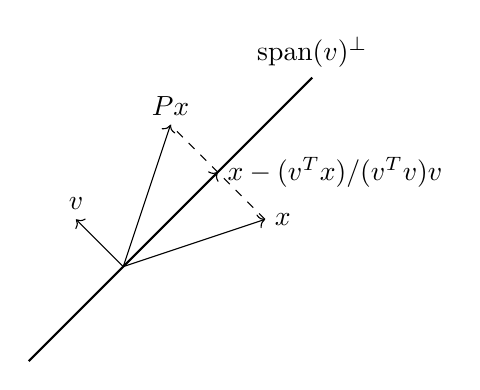
\begin{tikzpicture}[scale=0.6]
        \draw[->] (0,0) -- (-1,1) node[above] {$v$};
        \draw[->] (0,0) -- (3,1) node[right] {$x$};
        \draw[->] (0,0) -- (1,3) node[above] {$Px$};
        \draw[dashed] (3,1) -- (1,3);
        \draw[->] (0,0) -- (2,2) node[right] {$x - (v^T x)/(v^Tv)v $};
        \draw[thick] (-2,-2) -- (4,4) node[above] {${\rm span}(v)^\perp$};
    \end{tikzpicture}
    \caption{Householder矩阵作用在某一向量$ x $上}
    \label{fig:Householder}
\end{figure}

给定两个不同的向量$ x $和$ y $,如果它们的范数相同$ \| x \|_2 = \| y \|_2 $(因为$ P $是保矩的,所以范数相同是必要条件),我们可以通过Householder变换将$ x $变换为$ y $:令$ v = x - y $,则相应的Householder矩阵为
\[
    P = I - \frac{2(x - y)(x - y)^T}{(x - y)^T(x - y)} = I - \frac{2(x - y)(x - y)^T}{\| x - y \|_2^2},
\]
直接验证可知$ Px = y $。在实际应用中,通常令$ y $是一些具有特殊结构(有一些零)的向量,最常见的是令$ y = \sigma e_1 $,其中$ |\sigma| = \| x \|_2 $以保证相应的Householder矩阵是存在,此时的$ v = x - \sigma e_1 $,为了避免在计算两个相近的数相减时会出现的灾难性抵消现象(有效数字个数下降),通常令
\[
    \sigma = - {\rm sign}(x_1) \| x \|_2,
\]
于是$ v = x + {\rm sign}(x_1) \| x \|_2 e_1 $从而避免出现了减法;另一种做法如算法\ref{alg:Householder}所示,令$ \sigma = {\rm sign}(x_1) \| x \|_2 $,但是通过计算如下等价的公式来得到$ v $以避免减法的出现:
\begin{equation}\label{eq:Householder}
    v_1 = x_1 - \sigma = \frac{x_1^2 - \| x \|_2^2}{x_1+\sigma} = \frac{-(x_2^2 + \cdots + x_m^2)}{x_1+\sigma}.
\end{equation}

\begin{algorithm}[htbp]
    \caption{Householder Transform}\label{alg:Householder}
    \KwData{nonzero vector $ x\in \mathbb{R}^{n} $.}
    \KwResult{$ v $ and $ \beta = 2 / (v^Tv) $ s.t. $ Px = \sigma e_1 $ where $ P = I- \beta vv^T $, $ \sigma ={\rm sign}(x_1) \| x \|_2 $.}
    Preconditioning: $ \eta = \| x \|_\infty, \ x = x / \eta $\;
    $ (v_2,\cdots ,v_n) = (x_2,\cdots,x_n) $\;
    $ \alpha = (x_2,\cdots ,x_n)^T (x_2,\cdots ,x_n) $\;
    \eIf{$ \alpha = 0 $}{
        $ \beta = 0 $\tcc*[c]{$ x={\rm sign}(x_1)\| x \| e_1,\quad P=I $}
    }{
        $ \sigma = \sqrt{x_1^2 + \alpha} $\;
        \If{$ x_1\leqslant 0 $}{
            $ \sigma = -\sigma $\;
        }
        $ v_1 = -\alpha / (x_1+\sigma) $ \tcc*[c]{use \eqref{eq:Householder}}
        $ v = v / v_1 $ \tcc*[c]{normalize $ v $}
        $ \beta = 2 / (v^Tv) $\;
    }
    \Return $ v,\ \beta $\;
\end{algorithm}

算法\ref{alg:Householder}中最后一步令$ v $的首个元素标准化为$ 1 $,这一操作使得此时无需再储存$ v_1=1 $,所以可以直接将$ v_2,\cdots ,v_n $储存在$ Px $的后$ n-1 $个元素中(根据$ P $的构造,这些元素已知为0),这样可以节省一些内存。

下面我们使用Householder变换来实现QR分解。一般地,通过依次在$ A\in \mathbb{R}^{m\times n} $上左作用上$ n $个Householder矩阵,我们可以将$ A $变换为一个上三角矩阵$ R $。令$ A_1 = A $,如果在第$ k $阶段的开始得到的
\[
    A_k = 
    \begin{bmatrix}
        R_{k-1} & z_k & B_k\\
        0 & x_k & C_k
    \end{bmatrix},\quad R_{k-1}\in \mathbb{R}^{(k-1)\times (k-1)},\quad x_k\in \mathbb{R}^{m-k+1},
\]
其中$ R_{k-1} $是上三角矩阵,现在我们需要选取一个Householder矩阵$ \tilde{P}_k $,使得$ \tilde{P}_k x_k = \sigma e_1^{(k)} $,并且令
\[
    P_k = 
    \begin{bmatrix} 
         I_{k-1} & \\
         & \tilde{P}_k
    \end{bmatrix},
\]
于是得到的$ P_k A_k = A_{k+1} $的左上角有一个$ k $阶的上三角矩阵。继续这一过程就得到了$ A $的QR分解,其中
\begin{equation}
    R = P_n P_{n-1}\cdots P_1 A = Q^T A.
\end{equation}
这一过程总共需要进行$ 2n^2(m-n / 3) $次浮点运算。

在实际计算中,各个$ P_i $不会被显式地构造,出于存储和计算的效率考虑,我们只储存相应的$ v_i $来进行计算。例如在计算$ A_{k+1} = P_k A_k $时,由于
\[
    \begin{bmatrix} 
        I_{k-1} & \\
        & \tilde{P}_k
    \end{bmatrix}
    \begin{bmatrix}
         R_{k-1} & z_k & B_k\\
         0 & x_k & C_k
    \end{bmatrix} =
    \begin{bmatrix}
        R_{k-1} & z_k & B_k\\
        0 & e_1^{(k)} & \tilde{P}_k C_k
    \end{bmatrix},
\]
所以我们只需要更新$ C_k $到
\[
    \tilde{P}_k C_k = (I - \beta v_k v_k^T)C_k = C_k - \beta v_k(v^T_k C_k), \beta = \frac{2}{v^T_kv_k},
\]
其中我们通过利用矩阵乘法的结合律使用矩阵-向量积代替了矩阵-矩阵积,这一操作可以显著地减少计算量。

如果希望获得使得$ A=QR $的$ Q $矩阵,则需要计算$ Q = P_1 P_2\cdots P_n $,由于$ P_i $中有效的$ \tilde{P}_i $的阶数随着$ i $增长而减小,从右到左相乘相比于从左到右相乘更加高效。不过对于大多数应用而言,我们并不需要显式地计算$ Q $,只需要记录下各$ v_i $和最终得到的$ R $即可。

\begin{algorithm}[htbp]
    \caption{QR factorization by Householder Transform}\label{alg:HouseholderQR}
    \KwData{$ A\in \mathbb{R}^{m\times n} $ of rank $ n \ (m\geqslant n) $. }
    \KwResult{QR factorization of $ A $.}
    \For{$ j=1:n $}{
        \If{$ j<m $}{
            $ [v_j,\beta_j] = \text{Householder}(A(j:m,j)) $ \tcc*[c]{use algorithm \ref{alg:Householder}}
            $ A(j:m,j:n) = A(j:m,j:n) - \beta v_j(v_j^TA(j:m,j:n)) $\;
            $ A(j+1:m,j) = v_j(2:m-j+1) $\;
        }
    }
    \Return {$ R = {\rm triu}(A) $ (upper triangluar part of A), $ \beta\in \mathbb{R}^{n} $, $ v_j\in \mathbb{R}^{m-j+1} $ is stored in $ j $th column of $ {\rm stril}(A) $ (strict lower triangluar part of A) with first elemet being $ 1 $}\;
    \KwCost {$ 2n^2(m - n / 3) $ flops.}
\end{algorithm}

由于在第$ i $个阶段将$ A $的第$ i $列下方变为零之后就不再需要原本$ A $这一列了,因此没必要继续保留$ a_i $只需要储存这一过程中用到的Householder变换($ v_i $和$ \beta $)和得到的$ r_i $。出于这一原因,在算法\ref{alg:HouseholderQR}中,我们将每次用于生成Householder矩阵的$ v_j $(第一个分量为1无需储存,只需储存后$ m-j $个分量)储存在$ A $的严格下三角部分($ A(j+1:m,j) $)中,将$ r_i $(后$ m-j $个分量均为零无需储存)储存在$ A $的上三角部分($ A(1:j,j) $)中,$ \beta $额外储存在一个向量中,如下式所示($ A\in \mathbb{R}^{4\times 3} $的例子),其中$ v_j = (1, v_{j+1,j},\cdots ,v_{mj})^T $。
\[
    A\longrightarrow
    \begin{bmatrix} 
        r_{11} & r_{12} & r_{13}\\
        v_{21} & r_{22} & r_{23}\\  
        v_{31} & v_{32} & r_{33}\\
        v_{41} & v_{42} & v_{43}\\
    \end{bmatrix},
    \quad \beta =
    \begin{bmatrix}
        \beta_1\\
        \beta_2\\
        \beta_3
    \end{bmatrix}.
\]

\subsubsection{基于Householder变换的QR分解稳定性}
总的来说,Householder变换在数值上是相当稳定的:无论是对某个向量进行Householder变换,还是计算Householder变换矩阵与其他矩阵的乘积,在范数意义下都是稳定的,并且最重要的基于Householder变换的QR分解在范数意义下也是后向稳定的。

为了方便起见,定义
\[
    \tilde{\gamma}_k = \frac{cku}{1-cku},
\]
其中$ c $是某个较小的常数。

\subsection{Givens旋转}
Givens旋转是另一种进行QR分解的方法,它通过不断地向矩阵$ A $中引入零元素来得到上三角结构以实现QR分解,为此需要构造Givens矩阵$ G(i,j,\theta)\in \mathbb{R}^{n\times n} $($ i\ne j $),该矩阵形如
\[
    G(i,j,\theta) = 
    \begin{bmatrix}
        I_{\min\{i,j\}-1} & & & &\\
        & c & & s &\\
        & & I_{|i-j|-1} & &\\
        & -s & & c & \\
        & & & & I_{n-\max\{i,j\}}
    \end{bmatrix},
\]
它的第$ i,j $行和$ i,j $列相交构成的$ 2\times 2 $子矩阵如下所示:
\[
    G([i,j], [i,j]) = 
    \begin{bmatrix}
        c & s\\
        -s & c
    \end{bmatrix},
\]
其中$ c=\cos \theta, s= \sin \theta $,其他的元素与单位矩阵$ I_n $相同。从几何上看,$ y = G(i,j,\theta)x $是将$ x $在平面$ {\rm span}(e_i,e_j) $内顺时针旋转$ \theta $后得到的向量,即
\[
    \begin{bmatrix} 
        y_i \\ y_j
    \end{bmatrix} = 
    \begin{bmatrix}
        c & s\\
        -s & c
    \end{bmatrix}
    \begin{bmatrix}
        x_i \\ x_j
    \end{bmatrix},\quad y_{k} = x_k\ (k\ne i,j).
\]
为了令旋转之后的$ y_j =0 $,需要令
\begin{equation}
    s = \frac{x_j}{\sqrt{x_i^2 + x_j^2}},\quad c = \frac{x_i}{\sqrt{x_i^2 + x_j^2}},
\end{equation}
此时$ y_i = cx_i+sx_j $。上式说明要构造$ G(i,j,\theta) $只需要$ x_i,x_j $,无需计算出角度$ \theta $,因此也简记$ G(i,j,\theta) = G_{ij} $。使用这一方法可以依次的令矩阵的下三角区域的元素变为零从而最终得到一个上三角矩阵$ R $。


\begin{algorithm}[htbp]
    \caption{Givens Rotation}\label{alg:Givens}
    \KwData{$ a,b\in \mathbb{R} $.}
    \KwResult{$ c,s $ s.t. $ \begin{bmatrix} 
        c & s\\
        -s & c
    \end{bmatrix} 
    \begin{bmatrix} 
        a \\ b 
    \end{bmatrix} = 
    \begin{bmatrix} 
        r \\ 0
    \end{bmatrix} $.}
    \eIf{$ b=0 $}{
        $ c=1,\ s=0 $\;
    }{
        \eIf{$ |b|>|a| $}{
            $ \tau = a/b,\ s = 1/\sqrt{1+\tau^2},\ c = s\tau $ \tcc*[c]{avoid near 0 division}
        }{
            $ \tau = b/a,\ c = 1/\sqrt{1+\tau^2},\ s = c\tau $ \tcc*[c]{avoid near 0 division}
        }
    }
    \Return $ c,s $\;
\end{algorithm}

注意到如果$ i_1, i_2,j_1,j_2 $互不相同,则$ G_{i_1,j_1}G_{i_2,j_2} = G_{i_2,j_2}G_{i_1,j_1} $可交换,此时称$ G_{i_1,j_1} $和$ G_{i_2,j_2} $是不相交的。当$ G_{i_1,j_1} $和$ G_{i_2,j_2} $不相交时,$ G_{i_2,j_2}G_{i_1,j_1}A $可以并行地计算:
\[
    A([i_1,j_1],[i_1,j_1]) \leftarrow G_{i_1,j_1}A([i_1,j_1],[i_1,j_1]),\quad A([i_2,j_2],[i_2,j_2]) \leftarrow G_{i_2,j_2}A([i_2,j_2],[i_2,j_2]),
\]
因此Givens旋转法可以按照如下顺序并行地计算QR分解:
\[
    \begin{bmatrix} 
        \times & \times & \times & \times & \times\\
        1 & \times & \times & \times & \times\\
        2 & 3 & \times & \times & \times\\
        3 & 4 & 5 & \times & \times\\
        4 & 5 & 6 & 7 & \times\\
        5 & 6 & 7 & 8 & 9
    \end{bmatrix} 
\]
上述矩阵中某位置上的数字为$ k $表示在第$ k $步时使用Givens旋转将该位置上的元素变为零,具有相同数字的位置($ i+j $是确定的正数)可以并行地同时使用不相交的Givens旋转将其上的元素变为0($ i,j\ (i>j)$位置对应的Givens旋转为$ G_{i,j} $)。对于$ m\times n\ (m>n) $的矩阵,使用这种计算方法需要$ r=m+n-2 $各阶段,每个阶段最多并行地计算$ n $个Givens旋转,最终得到$ R = W_rW_{r-1}\cdots W_1 A $,$ W_i $最多是$ n $个Givens旋转矩阵的乘积。

\begin{algorithm}[htbp]
    \caption{QR factorization by Givens Rotation}\label{alg:GivensQR}
    \KwData{$ A\in \mathbb{R}^{m\times n} $ of rank $ n \ (m \geqslant  n) $. }
    \KwResult{QR factorization of $ A $.}
    \For{$ k=1:m+n-2 $}{
            \If{$ m=n \text{ and } k=m+n-2 $}{
                Break out \tcc*[c]{square martix need only $ m+n-3 $ steps}
            }
            \tcc{Find the border element of the matrix to be zeroed in this step}
            \eIf{$ k+1>m $}{
                $ i = m,\ j = k+2-m $ \tcc*[c]{the last row}
            }{
                $ i = k+1,\ j = 1 $ \tcc*[c]{the first column}
            }
            \tcc{Introduce zeros in the anti-diagonal manner}
            \For{$ l = 0: \min(\lceil \frac{i-j-1}{2} \rceil, n) $}
            {
                \tcc{this loop can be parallelized}
                $ [c,s] = \text{Givens}(A(j+l,j+l),A(i-l,j+l)) $ \tcc*[c]{algorithm \ref{alg:Givens}}
                $ A(j+l,j+l:n) = cA(j+l,j+l:n) + sA(i-l,j+l:n) $\;
                $ A(i-l,j+l+1:n) = -sA(j+l,j+l+1:n) + cA(i-l,j+l+1:n) $\;
                $ A(i-l,j+l) = c + s \text{i} $ \tcc*[c]{$ e^{i\theta} $, $ c,s $ are real and complex part of $ e^{i\theta} $}
            }
        }
    \Return $ R = {\rm triu}(A),\ C = {\rm Re}({\rm stril}(A)),\ S = {\rm Im}({\rm stril}(A)) .$\;
\end{algorithm}

算法\ref{alg:GivensQR}中,我们直接将用于构造Givens旋转的$ C $和$ S $储存在$ A $的严格下三角部分中,最终得到的$ R $则储存在$ A $的上三角部分中。其中$ \lceil \frac{i-j-1}{2} \rceil $是不大于$ (i-j-1)/2 $的最大整数。

\subsection{Gram-Schmidt正交化}
Gram-Schmidt正交化可以将一组线性无关的向量$ \{v_1,\cdots ,v_n\} $变为一组标准正交的向量$ \{u_1,..,u_n\} $,这一方法的基本思想是通过逐次地从某一向量中减去它在前面的向量上的投影来实现正交化,基本步骤为令$ u_1 = w_1 / \| w_1  \|_2 $,其中$ w_1=v_1 $,对于$ i = 2,\cdots ,n $,令
\[
    w_i = v_i - \sum_{j=1}^{i-1} \frac{v_i^T w_j}{u_j^T w_j}w_j = v_i - \sum_{j=1}^{i-1} (v_i^T u_j)u_j ,\quad u_i = w_i / \| w_i \|_2.
\]

对于$ m\times n\ (m\geqslant n) $的矩阵$ A $,我们可以对$ A $的各列向量使用Gram-Schmidt正交化方法,于是根据以上的算法
\[
    a_i = \sum_{j=1}^{i-1}(a_i^T u_j)u_j + \| w_i \|_2 u_i,
\]
因此
\[
    A = [a_1, a_2, \cdots , a_n] = [u_1, u_2, \cdots , u_n] 
    \begin{bmatrix}
        \| w_1 \|_2 & a_2^T u_1 & \cdots & a_n^T u_1\\
        & \| w_2 \|_2 & \cdots & a_n^T u_2\\
        & & \ddots & \vdots\\
        & & &\| w_n \|_2
    \end{bmatrix},
\]
就是$ A $的QR分解,每一个阶段我们得到$ Q $和$ R $的一列元素,这就是如算法\ref{alg:CGS}所示的经典Gram-Schmidt正交化算法(CGS)。

\begin{algorithm}[htbp]
    \caption{Classic Gram-Schmidt Procedure}\label{alg:CGS}
    \KwData{$ A = (a_1,\cdots ,a_n)\in \mathbb{R}^{m\times n} $ of rank $ n \ (m\geqslant n)$. }
    \KwResult{QR factorization of $ A $.}
    Initialize: $ r_{11} = \| a_1 \|_2,\ q_1 = a_1 / r_{11} $\;
    \For{$ j=2:n $}{
        \For{$ i=1:j-1 $}{
            $ \textcolor{blue}{r_{ij} = q_i^T a_j} $ \tcc*[c]{Projection}
        }
        $ q'_j = a_j - \sum_{k=1}^{j-1} r_{kj}q_k $ \tcc*[c]{Orthogonalization}
        $ r_{jj} = \| q'_j \|_2 $\;
        $ q_j = q'_j/r_{jj} $ \tcc*[c]{Normalization}
    }
    \Return $ Q = (q_1,\cdots ,q_n)\in \mathbb{R}^{m\times n},\ R=(r_{ij})\in \mathbb{R}^{n\times n} $\;
    \KwCost {$ 2mn^2 $ flops.}
\end{algorithm}
通过对CGS的计算过程重新排序可得如算法\ref{alg:MGS}所示的修正Gram-Schmidt正交化算法(MGS)。
\begin{algorithm}[htbp]
    \caption{Modified Gram-Schmidt Procedure}\label{alg:MGS}
    \KwData{$ A = (a_1,\cdots ,a_n)\in \mathbb{R}^{m\times n} $ of rank $ n \ (m\geqslant n)$. }
    \KwResult{QR factorization of $ A $.}
    Initialize: $ a_k^{(1)} = a_k $ for $ k=1,2,\cdots ,n $\;
    \For{$ k=1:n $}{
        $ r_{kk} = \| a_k^{(k)} \|_2 $\;
        $ q_k = a^{(k)}_k / r_{kk} $\;
        \For{$ j=k+1:n $}{
            $ \textcolor{red}{r_{kj} = q_k^T a_j^{(k)}} $ \tcc*[c]{MGS use partially orthogonalized $ a_j^{(k)} $ instead of $ a_j $}
            $ a_j^{(k+1)} = a_j^{(k)} - r_{kj}q_k $ \tcc*[c]{Partial orthogonalization}
        }
    }
    \Return $ Q = (q_1,\cdots ,q_n)\in \mathbb{R}^{m\times n},\ R=(r_{ij})\in \mathbb{R}^{n\times n} $\;
    \KwCost {$ 2mn^2 $ flops.}
\end{algorithm}

在CGS中,每经过一次外层循环,我们就得到$ Q $的一列元素和$ R $的一列元素,而在MGS中,每经过一次外层循环就需要对$ Q $的后几列都进行一次更新,同时得到$ R $的一行元素。换言之,CGS每层外循环的作用只是将当前列变为与之前的列都正交的单位向量,不去管后面的各列;MGS每层外循环则是在得到一列与之前的所有列都正交的单位向量之后,还要将后续的列在该新得到的单位向量上的投影也都减去(后续列都被\emph{部分正交化}),即在第$ i $次外循环中,首先获得了第$ i $个与之前向量都正交的单位向量$ q_i = a^{(i)}_i $,然后还要令
\[
    a^{(i+1)}_j = a_j^{(i)} - (a_j^{(i)}, q_i)q_i,\quad j = i+1,\cdots ,n,
\]
这样一来,为了保证正交性而减去投影的操作就被分散在了多次循环中,而不像CGS那样在一次循环中完成。

尽管CGS和MGS在数学上是相同的,后者只不过是前者在以另一种顺序进行计算,但是在进行数值计算时,由于浮点计算会引入误差,此时通过MGS得到的矩阵$ Q $的正交性往往远远优于CGS,这主要是因为两者得到$ r_{kj} $的方式不同:在CGS中$ r_{kj} = q_k^T a_j $只与$ A $的一列$ a_j $有关,而在$ MGS $中使用的是$ r_{kj} = q_k^T a_j^{(k)} $,其中的$ a_j^{(k)} $是已经被部分正交化之后的$ a_j - \sum_{i=1}^{k-1}(a_j,q_i)q_i $,因此之前的正交化误差$ (q_i,q_j) $不会累积到$ r_{kj} $的计算中。基于以上原因,如果希望得到的$ Q $具有较好的正交性,则MGS是比CGS更好的选择。

\section{最小二乘问题}

\subsection{使用QR分解求解最小二乘问题}

\subsection{使用MGS求解最小二乘问题}

\subsection{误差分析}

\section{特征值问题}

\subsection{幂法和反幂法}

\subsection{QR算法}

\subsection{奇异值分解}

\bibliography{Lib}
\end{document}